% !TEX root = main.tex
\chapter{Design and simulation of the addressing setup}
The purpose of this thesis work was to develop a single-ion-addressed laser system for the purpose of generating single photons and for single ion-qubit control. In this chapter we discuss the design and the implementation of such setup. The design is a crucial part of the work, since there are several requirements that have to be met in order to achieve the proper needed functionalities. In the first section, the requirements are presented together with an overview of the design idea. In the setup an objective was already present, and the choice of an AOD was already made, in anticipation of my project. Hence, we discuss these components as given. The rest of the setup was simulated with the software Zemax, which was used to find the optimal optical components and their placement.
\section{Addressing system overview and requirements}
\label{sec:addressing}
Single-ion addressing laser systems have already been developed and employed in experiments successfully. The main idea is to focus a laser beam tighter than ion-ion separation and steer it between different ions on a few micro-second timescale. In Innsbruck calcium ions have been addressed in this way, where the steering was achieved with an AOD \cite{addressing}; At Duke university, laser beams have also been steered with micro-electromechanical systems (MEMS) mirrors \cite{addressing3}. Another idea is to send a normal beam illuminating all the ions, but hiding those who are not addressed. This was done with Ytterbium atoms where by means of a inhomogeneous magnetic field the transition frequencies were shifted shielding selected ions \cite{addressing2}. \\
Our choice was to implement the approach of Innsbruck with an AOD and improve it. The advantage of AODs is to have a switching time in the order of $\mu$s, that is used for fast switching between ions. A problem with the implementation of \cite{addressing} is limited addressing range as the beam clips on the edge of optics when working with strings of ten ions or more at typical confinement. Furthermore, their system is developed for 729 nm light, while our goal is excite the 393 nm transition, this requires new simulations and different optics. Therefore, the new designed system aims to exploit the full capabilities of the AOD while maintaining a very tight focus. In order to achieve this, there are two aspects to keep in mind: the focus spot, and the addressing range. However the priority was the focus spot as experiments planned in our team involve only a handful of ions in the foreseeable future.
\begin{figure}[H]
\centering
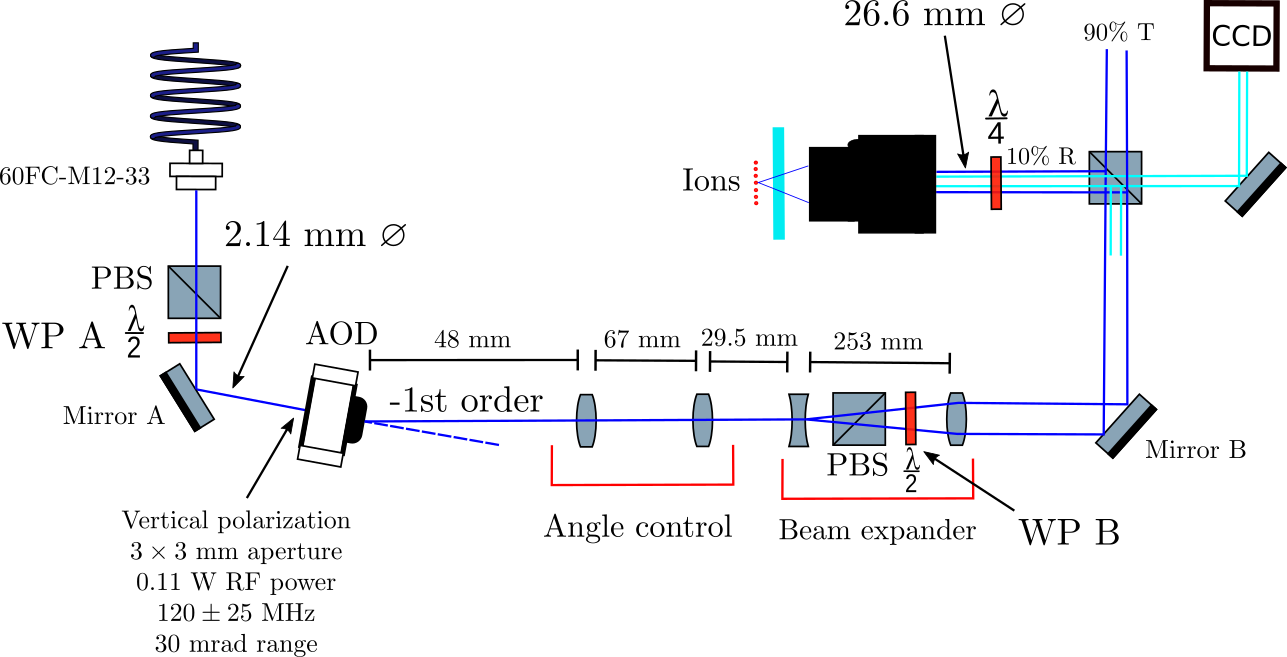
\includegraphics[width=\textwidth]{img/setup}
\caption{Scheme of the setup. Light comes from a fiber, polarization is cleaned, and then sent thorough the AOD from Gooch \& Housego 4120-3. -1st order diffracted light is refocused into a beam expander, where the beam is broadened before being focused by the objective. All lenses are from Thorlabs, models are from left to right: LA-1059, LA-1131, LA-4252, LA1725; all of them are AR coated for 393 nm. Critical distances between lenses are in the figure, distance between last lens and objective is 722 mm. The 90:10 Beam splitter is custom made by Laser Components GmbH. Diameters $\varnothing$ are expressed as $1/e^2$ of intensity. Between objective and ions there is a 6 mm thick glass of the viewport, as the objective is out of vacuum. $\lambda/2$ waveplates are labeled as WP A, and WP B for future reference. Light blue lines represents 397 nm light coming from the ions into the imaging setup.}
\label{addressingsetup}
\end{figure}
The addressing setup should be able to address single ions in a string in order to generate single photons out of single ions via the already discussed Raman process. Ion separations, in the case of two $^{40}\text{Ca}^+$, has been derived in section \ref{ionstrings}, for a axial center of mass frequency of 1 MHz is 5.6 $\mu$m. The setup must therefore be able to focus a laser beam down to 1-2 $\mu$m waist to essentially eliminate cross talk. As seen in section \ref{sec_diffraction}, a tighter focus can obtained with a shorter wavelength, a bigger lens, or with a shorter focal length. The focusing lens, a.k.a the objective, is shared with the imaging setup, and thus it is given, the focal length is therefore a constant in the problem, see section \ref{sec:obj}. The wavelength is also a constant, as the Raman process happens at 393 nm. This gives only one possibility left to tighten the focus, i.e. by making the beam as broad as possible at the objective input surface.\\
Figure \ref{addressingsetup} presents the final layout of the addressing setup. Some key aspects are now discussed. Beam expansion is achieved with a Galilean telescope, it takes two lenses to form such Telescope, a concave lens to diverge a collimated beam and a convex lens to collimate the diverging beam. The combination of these two lenses takes a collimated beam and expand it to another collimated beam with an expansion factor of 23.9\footnote{Since the beam is not collimated after the beam expander, the expansion factor has been calculated as the ratio of the incoming and outgoing beam diameters of the beam expander.}. This expansion part is one of the two essential part of the addressing setup. The other part is related to the addressing spatial range. Not only, we want to focus the beam to a single ion, but we want to move the beam as well, such that it focuses on a different ion. Therefore, there is a requirement also on the range that can be addressed. This depends on the number of ions and their spacing, we chose to aim to address many tens of ions, this requires the ability to move the focus along the ion string by 150-200 $\mu$m. Beam steering is possible with the use of an AOD, the detailed working principle of this device has been discussed in section \ref{theory_AOD}. Basically the angle of the output beam of the AOD changes as the driving frequency changes. However, the AOD must be placed far behind the objective to leave space for the beam expander, this implies a need to control and redirect the angle of the AOD's output beam to send it to the beam expander and later in the objective without any clipping. This task is accomplished with a pair of converging lenses (Angle control in figure \ref{addressingsetup}), they refocus the collimated beam into the beam expander, beam then becomes wider, reaches the objective and it is focused on the ion. It is important to get the right lenses at the right distances, the objective has 5 different lenses inside, see section \ref{sec:obj}. The objective was not designed to focus incoming collimated blue light onto the ions, but rather to image photons from the ions onto a camera 1.5 m away from the objective. Simulations showed that a slightly diverging 393nm beam ($\sim 0.5^\circ$), incoming into the objective, will be focused onto the ions. As such, we set the telescope to expand the beam without collimating it, leaving it diverging, so that the objective can focus it at the right position.\\
The setup displayed in figure \ref{addressingsetup} also contains polarization optics. As discussed in section \ref{sec:ramanprocess}, Zeeman transitions are polarization sensitive, thus polarization control is required. The AOD is polarization sensitive, which means it requires a certain input polarization and outputs another particular polarization, that is the reason why half wave plate are before and after, and additional quarter wave plate is inserted before the objective to obtain circular polarized light. This placement means having a bigger plate than standard, but if placed before in the optical path, the mirror and the beam splitter could alter the polarization. Moreover, the quarter wave plate is zeroth order and custom made, in order to have a greater polarization stability.\\
The choice of using a 90:10 beam splitter (figure \ref{addressingsetup}) to overlap the incoming 393 nm addressing laser with the outgoing 397 nm ion fluorescence for imaging is unusual, a common choice is to use a dichroic mirror. However, the light in the imaging path is 397 nm, very close to the 393 nm light of the addressing setup. This would have meant using a very narrow dichroic, the alternative was to use a 90:10 beam splitter, where 90\% of the light is transmitted and only 10\% of the light is reflected. In this way, only 10\% of imaging light is lost, at cost of 90\% of addressing laser light, which is not a problem as power is available. Furthermore, this light is focused so tightly that even a small amount of light can excite the ions. On the other end, it is not so straightforward to get more scattered light from the ions, so 397 nm light and the imaging setup must be as efficient as possible, with 10\% of losses, ions are still visible on the camera.

\section{Objective and AOD}
\label{sec:obj}
% \begin{figure}[H]
%      \centering
%      \begin{subfigure}[b]{0.4\textwidth}
%          \centering
%          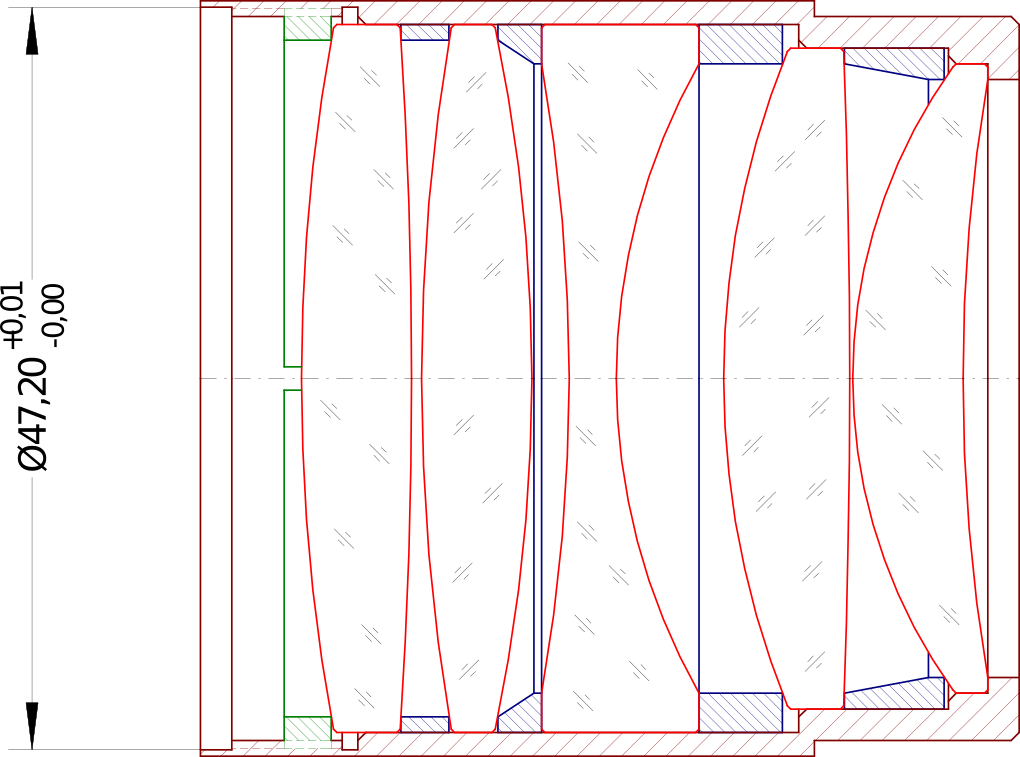
\includegraphics[width = \textwidth]{obj}
%           \caption{Section of the custom objective, red parts are the lenses, while the rest is the housing.}
%          \label{objsection}
%      \end{subfigure}
%      \hfill
%      \begin{subfigure}[b]{0.55\textwidth}
%          \centering
%          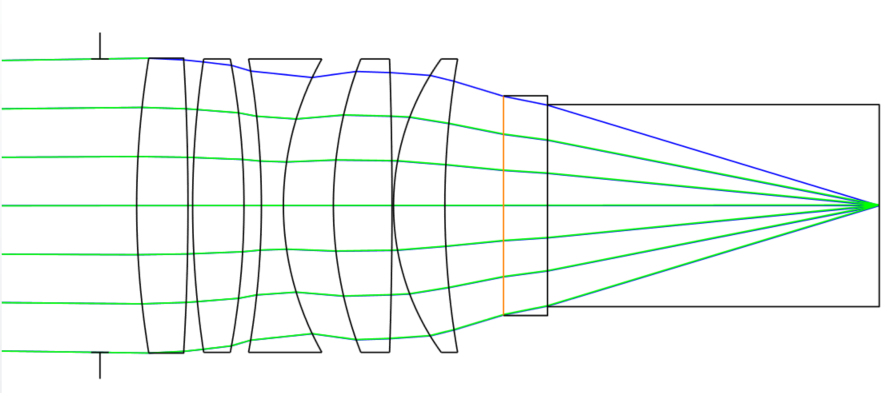
\includegraphics[width=\textwidth]{zeemaxobj}
%          \vspace{1em}
%          \caption{Zemax simulation of the objective. On the right, viewport and the vacuum chamber are also present.}
%          %\label{fig:three sin x}
%
%      \end{subfigure}
%         \caption{}
%       %  \label{fig:three graphs}
% \end{figure}
\begin{figure}[H]
      \centering
          \centering
          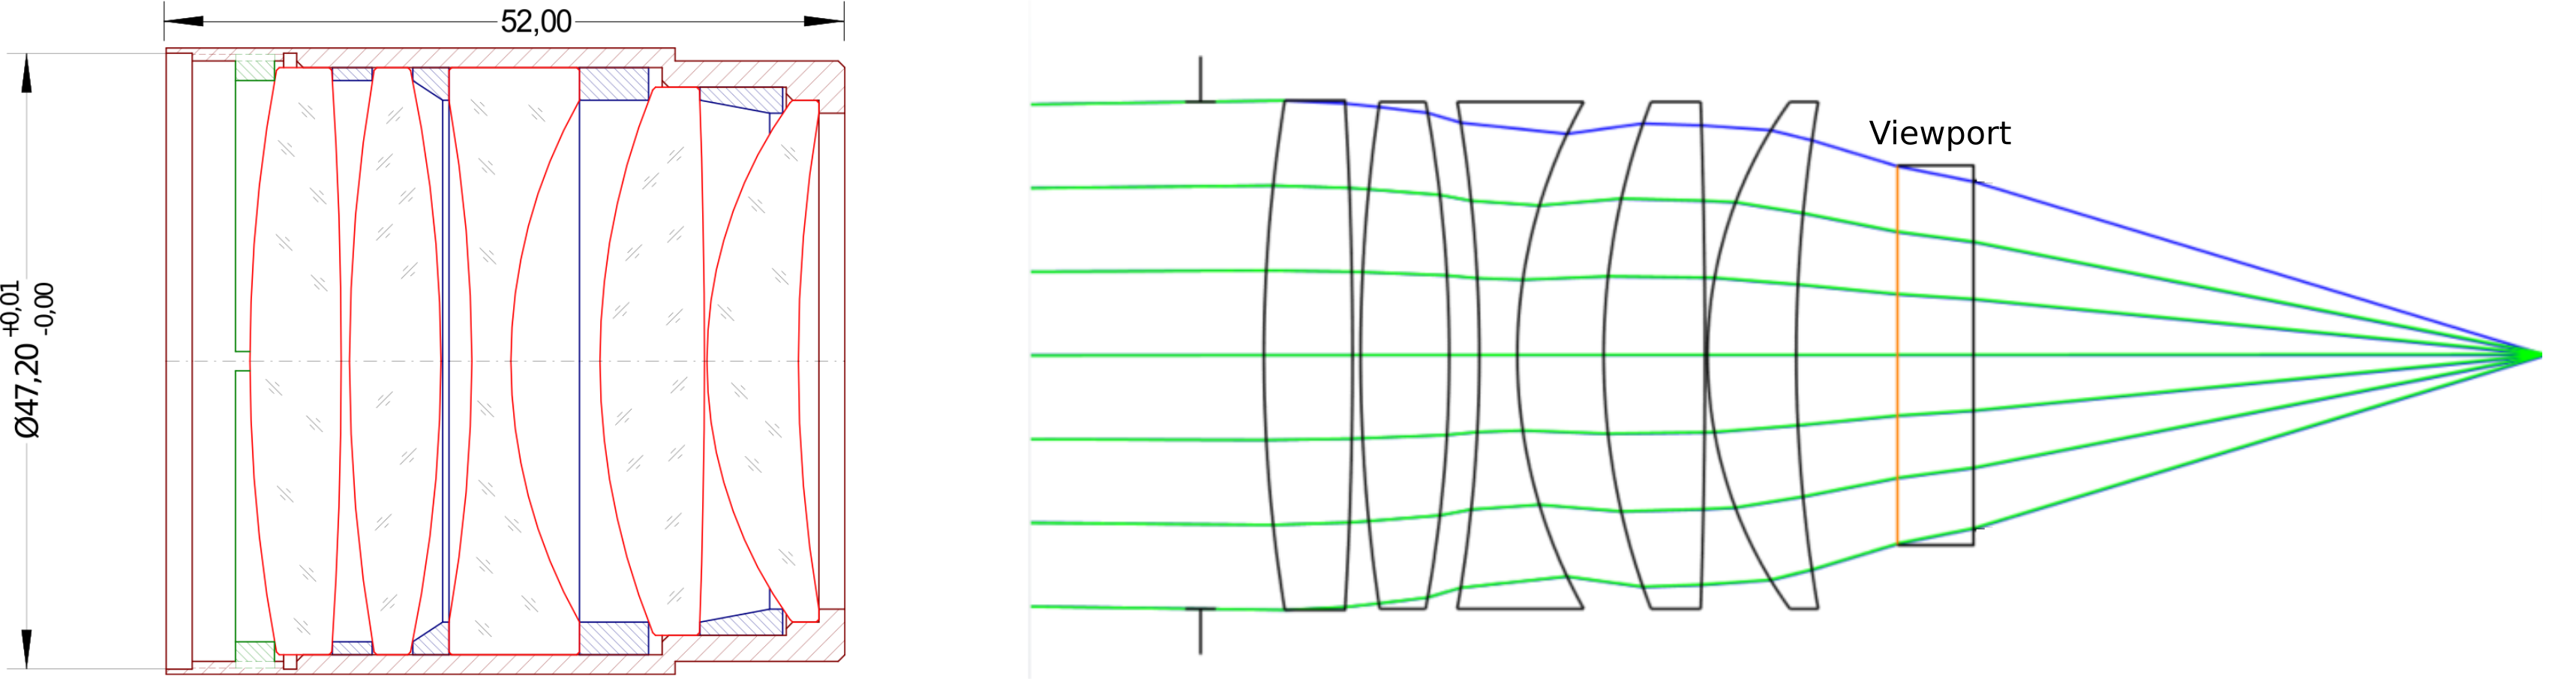
\includegraphics[width = \textwidth]{obj+zemaxpng}
           \caption{On the left, section of the custom objective made by Sill Optics, in red the 5 lenses are depicted, while the rest is the mechanical housing, given dimensions are in mm. On the right, Zemax simulation of the objective, viewport is also included.}
          \label{objsection}
\end{figure}
The objective used to focus the light was already present in the system and had to be taken as it is. It is a custom objective by Sill optics placed outside vacuum, in figure \ref{objsection} depiction of the objective and Zemax simulation are present.\\
This objective has different purposes, it was designed keeping in mind: imaging of ions by collecting 397 nm photons from ions, and imaging them onto a spot 1.5 meters away from the chamber; single-ion focusing with 729 nm light. Every lens is AR coated, the numerical aperture is NA = 0.289, thus effective focal length $f = 66.8$ mm. Furthermore, the objective was also designed to take into consideration the fact that it is placed out of vacuum, the light after the objective has to go through a 6 mm fused silica viewport and a further 38.6 mm of vacuum before reaching the ions. The objective is also mounted on a 3 dimensional translational stage to allow for imaging and addressing calibration.\\
The AOD is from Gooch \& Housego, model 4120-3, the datasheet is in Appendix \ref{sec:aoddata}. All the following parameters are specified in the datasheet, measured values are found in section \ref{sec:resultaod}. The crystal is Tellurium dioxide (TeO$_2$), the company specifies a central frequency of 120 MHz, with 50 MHz, bandwidth, so the driving frequency ranges from 95 to 145 MHz with a maximum RF power of 0.3 W. Addressing spatial range of 30 mrad, i.e. angle of deflection $\pm 0.86^{\circ}$. In this bandwidth the diffraction efficiency should remain above 75 \% and have an average of 83 \%, further 3\% of light is lost due to insertion losses. The active aperture measures $3\times 3$ mm, and the polarization has to be horizontal when entering the AOD, while the specified output polarization is vertical.

\section{Design simulation}
The setup in figure \ref{addressingsetup} has been simulated with the software Zemax\footnote{Zemax OpticStudio is a commercial software based on ray tracing used for designing optical system.}. The simulation had the purpose of assessing the performance of the setup, i.e. checking the viability of the setup and see if it meets all requirements. It was also used to find suitable lenses for building the setup and their optimal locations. The simulation included: the four lenses, the objective, and the viewport. As there is no option to simulate an AOD, it was not taken in consideration, instead the simulation started at the output of the AOD as described below. Mirrors and beam splitters were not included in the simulation as their imperfections are not currently known.
\begin{figure}[H]
\centering
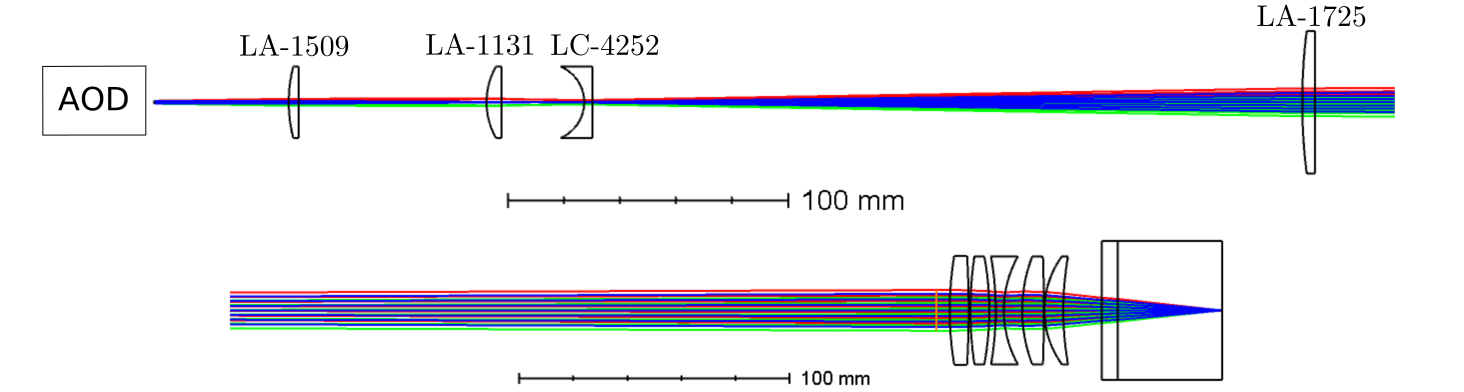
\includegraphics[width = \textwidth]{2levelszemax}
\caption{Zemax simulation of the setup. Rays propagate from left to right starting from top right. Simulation layout has been separated in two for displaying purposes. In the top part, the four lenses are depicted, the rays continue in the bottom part where the objective and image plane are located. Different colors indicate different beams emerging from the AOD at different angles, rays with the same color belong to the same beam. The blue one is the central beam emerging from the AOD with a 0$^\circ$ angle, the red and the green beams emerge respectively with $\pm0.86^\circ$.}
\label{zemaxview}
\end{figure}
The simulation starts by specifying the input fields, these represent the physical light beam. To account for the ability to change the output angle from the AOD, three different fields have been simulated. One is along the optical axis, while the other two are angled corresponding to the extrema of the AOD bandwidth, so $\pm0.86^{\circ}$. Therefore the propagation of these beams represents three different situations of beam direction and should also give an idea of the behavior in between the extrema. Next, the four lenses of the setup were inserted in Zemax, initially with variable radius, thickness and separations. Initial positions and lens focuses were set according to geometrical boundaries given by physical constraints on the optical table where the setup had to be built. The Zemax file of the objective came from the company which designed it and was simply imported in the project. After the objective the 6 mm viewport glass was included and then vacuum for 38.6 mm, which is the distance between the outer facet of the glass and the ion axis. The image plane was therefore set here. The distance between the objective and the viewport was unknown, as it could not be measured. However, this distance was inferred from a Zemax simulation of the imaging path, knowing that the ions focus on the camera 1.5 m away, we determined a space between the viewport and the objective of 14.22 mm.\\
The simulation was carried out with the tool Physical Optics Propagation (POP). POP works by propagating a wavefront represented by an array of discrete points. The array is propagated through every optical component and free space. This method can be used to simulate coherent Gaussian beams with high precision as well as wave phenomena such as diffraction and aberrations. The initial value given to the propagator was the waist of the collimated beam out of the AOD. Since the beam going to the AOD comes from a fiber collimator, the value specified was taken from the datasheet of the fiber collimator, namely Sc\"after + Kirchhoff 60FC-M12-33 \cite{fibercollimator}. Therefore, the specified waist was 1.07 mm.
\begin{figure}
     \centering
     \centering
     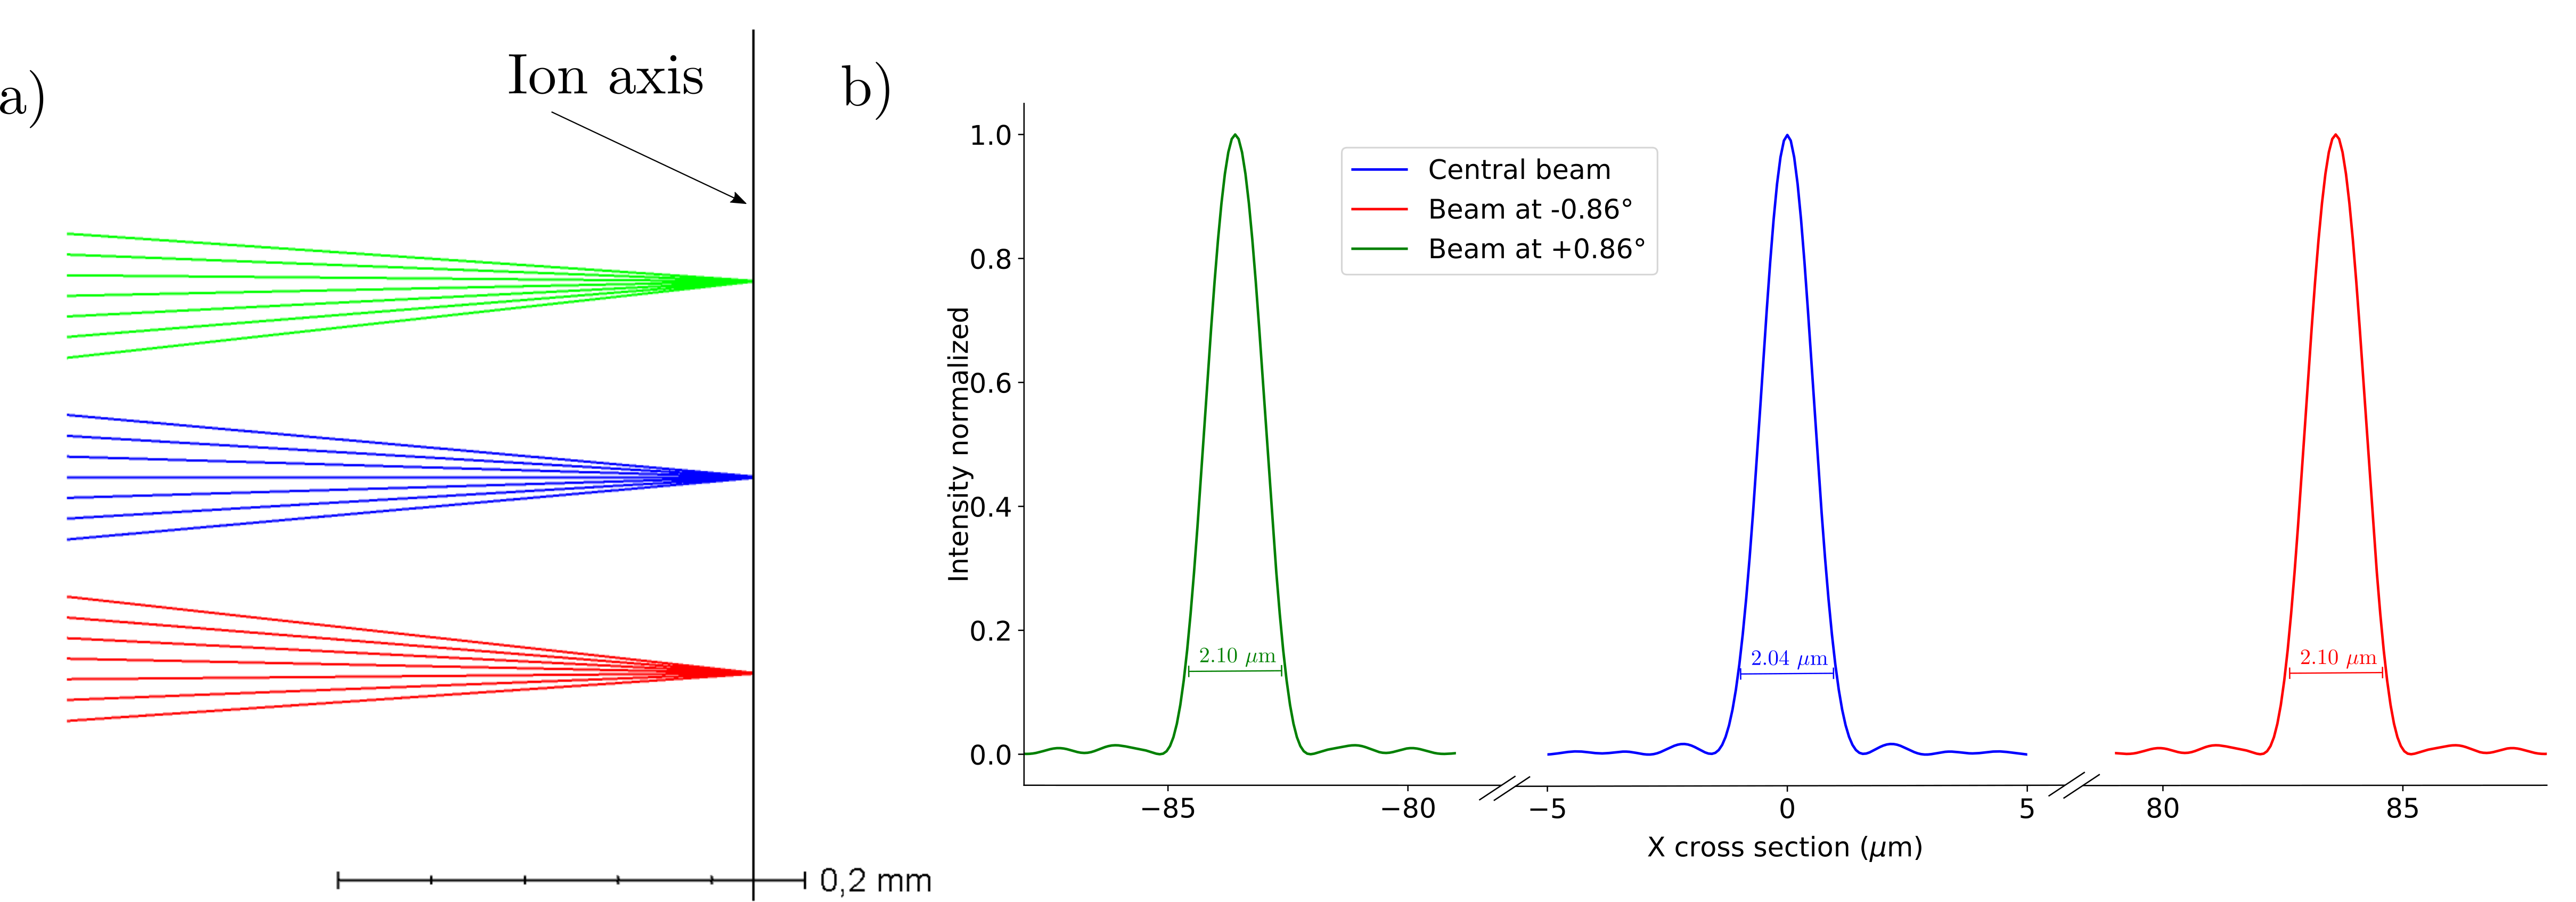
\includegraphics[width=1\textwidth]{img/range_plus_3beams}
     \caption{Zemax simulation at the image plane, where the ions are. a) Addressing range from Zemax simulation, the three beams emerge from the AOD at different angles. The full addressing range here displayed is 168 $\mu$m. b) Physical Optics Propagation of the three Gaussian beams with angles of $0,\pm0.86^\circ$, and waist at AOD of 1.07 mm. Displayed is the $x$ cross section at the ion axis. Beam diameters (13.5\%) are also displayed, the central beam at 2.04 $\mu$m is slightly narrower with respect to the outer ones $2.1$ $\mu$m.}
     \label{zemaxrange}
\end{figure}

The first step of the simulation work was to find the appropriate lenses to build the setup. The thicknesses and the radii were optimized trying to achieve the smallest focus spot while maintaining the desired addressing range. The lenses were found with the Zemax tool \emph{Stock Lens Matching}. Basically, the tool compares the simulated lenses with those in a catalogue from different companies and finds the closest match. We opted to rely on the provider Thorlabs, so the search was limited to this company. Found lenses were in order from left to right LA-1059, LA-1131, LA-4252, and LA-1725 and can be seen in figure \ref{zemaxview}. Once the desired lenses were found, their Zemax files provided by the company were imported in the project and further optimization was carried on.\\
The second step was to optimize the lenses position always trying to keep the focus spot as small as possible, and the desired addressing rage of 150-200 $\mu$m. This was done using the optimizing tools of Zemax and the merit function. The software can perform multivariate analysis and minimize the focus spot depending on all the assigned variables, which in this case were the distances between the lenses. The final results can be seen in figure \ref{zemaxrange}, the addressing range is 168 $\mu$m set by the bandwidth of the AOD from the specification sheet, while the waist of the central beam is $1.02\,\mu$m, beams at the border of the addressing range are $3\%$ broader, with a waist of $1.05$ $\mu$m.\\
Another important parameter for the performance of the setup is the addressing error. Qualitatively speaking, in the case of the beam focused on one ion, the addressing error is the leaking light on the neighbour ions. It can be a problem in the case of aberrations that produce bumps on the side of the main Gaussian peak. Especially in the case of diffraction limited system, the profile of the beam is a sinc function that can have more local maxima around the central peak. To estimate the addressing error in a simulation, two ions are placed next to each other at 5.6 $\mu$m, and the respective addressing beams have been simulated. The addressing error is different for different physical process, in the case of AC Stark shift, as the experiment discussed in \ref{sec:expqubit}, the shift is proportional to the intensity, so the addressing error is calculated as $I_1(x_2)/I_1(x_1) \simeq 10^{-4}$, where $I_{1}$ is the intensity profile of the beam focused on ion 1, and $x_1,x_2$ are respectively the position of ion 1 and ion 2. In the case of the cavity mediated Raman process, as in the experiment discussed in section \ref{sec:expphoton}, the strength of the process is proportional to the Rabi frequency, i.e. the electric field. Therefore, the addressing error is given as $\sqrt{I_1(x_2)/I_1(x_1)} \simeq 10^{-2}$.
 \begin{figure}
 \centering
 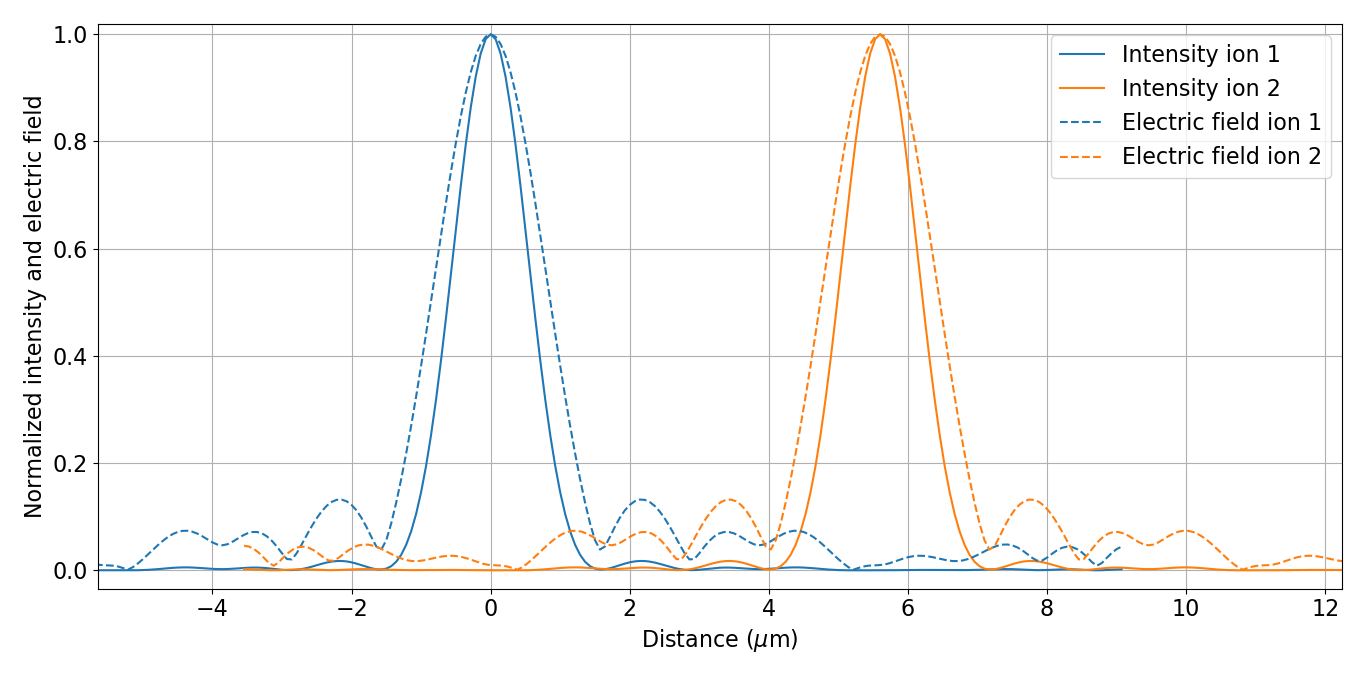
\includegraphics[width = .9\textwidth]{zemaxaddrerror3}
 \caption{Beam focused in two different places separated by 5.6 $\mu$m corresponding to the theoretical equilibrium positions of two ions with axial center of mass frequency of 1 MHz. Addressing error for AC Stark shift is calculated as the ratio of intensities at ion positions: $I_1(x_2)/I_1(x_1) \simeq 10^{-4}$. For Raman transition, the ratio of electric fields is taken: $\sqrt{I_1(x_2)/I_1(x_1)} \simeq 10^{-2}$.}
 \label{zemaxaddrerror.png}
 \end{figure}
Another aspect that was simulated is the beam profile inside the trap. Optical access to the trap is limited and a tightly focused beam also has a large divergence, which could lead to clipping on the trap's blades or compensation electrodes, scattering light all around the trap. In figure \ref{lossesplot} the top view of the trap is plotted, here we included the three pairs of compensation electrodes, the RF blades, and the cavity mirrors. The blue line represents the radius $W(z)$ from equation \ref{waistprofile} of the addressing beam in the case of a waist $W_0$ of 1 $\mu$m. To determine the fraction of power lost due to clipping on the compensation electrodes, we can calculated the transmitted power through the top electrodes:
\begin{equation}
P_{t} = \int_{-\infty}^{\infty}\text{d}y \int_{-x_c/2}^{x_c/2}\text{d}x P(z),
\end{equation}
where $P(z)$ is the power of the Gaussian beam, and $x_c$ is the horizontal position of the compensation electrode. The integral can be computed numerically at position $z$ of the electrodes. The result is plotted in figure \ref{lossesplot}, where the lost power $1-P_{t}$ is plotted as a function of the waist $W_0$. At the expected waist of $1.02\,\mu$m, the power lost is less than 1\%, i.e. for 2 $\mu$W AOD input power, after considering all the losses in the setup, it means losing less than a nW. The previous calculation holds only if the beam is perpendicular to the $x$ direction so it is important to align it carefully.
% \begin{figure}
%      \begin{subfigure}[b]{0.4\textwidth}
%           \centering
% 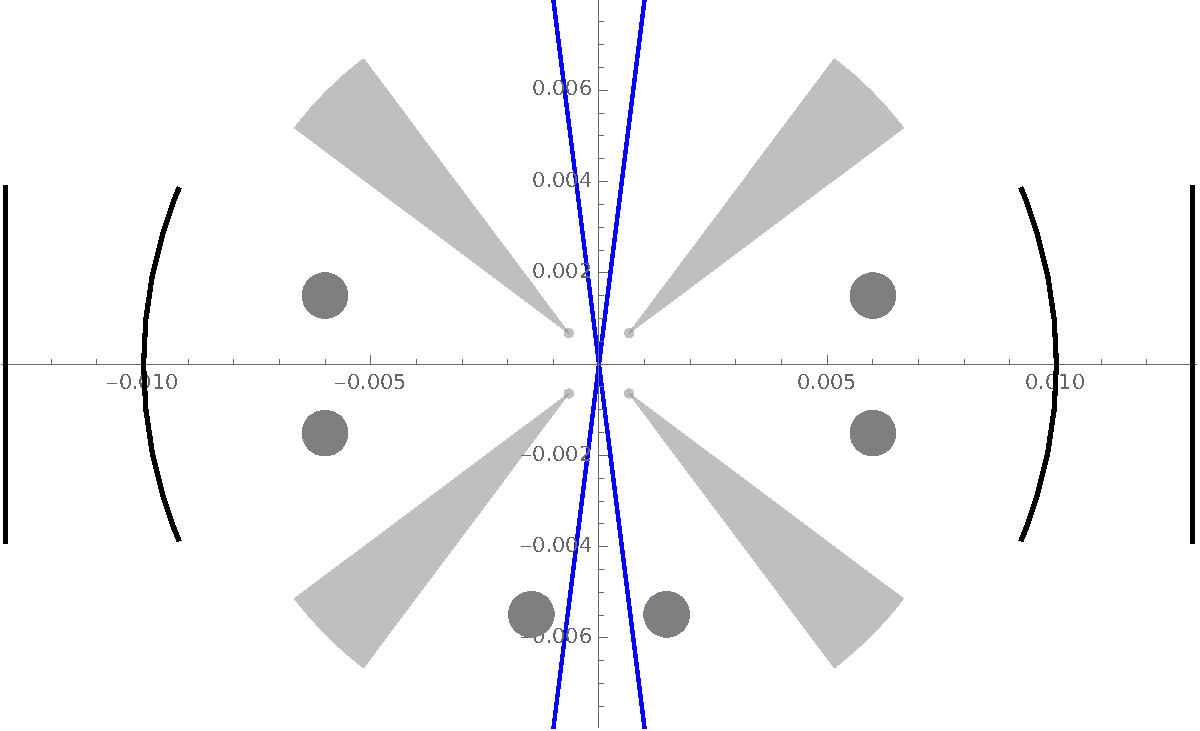
\includegraphics[width=.7\textwidth]{img/clipping}
%      \caption{Top view of the trap and addressing beam. Grey circles are the compensation electrodes, blue is the radius $1/e^2$ of the beam focused on the ions with waist of 1 $\mu$m, while the black arches represent the mirrors of the cavity. All units are in meters.}
%       \label{clippingtop}
%     \end{subfigure}\hfill
%     \begin{subfigure}[b]{0.49\textwidth}
%          \centering
%          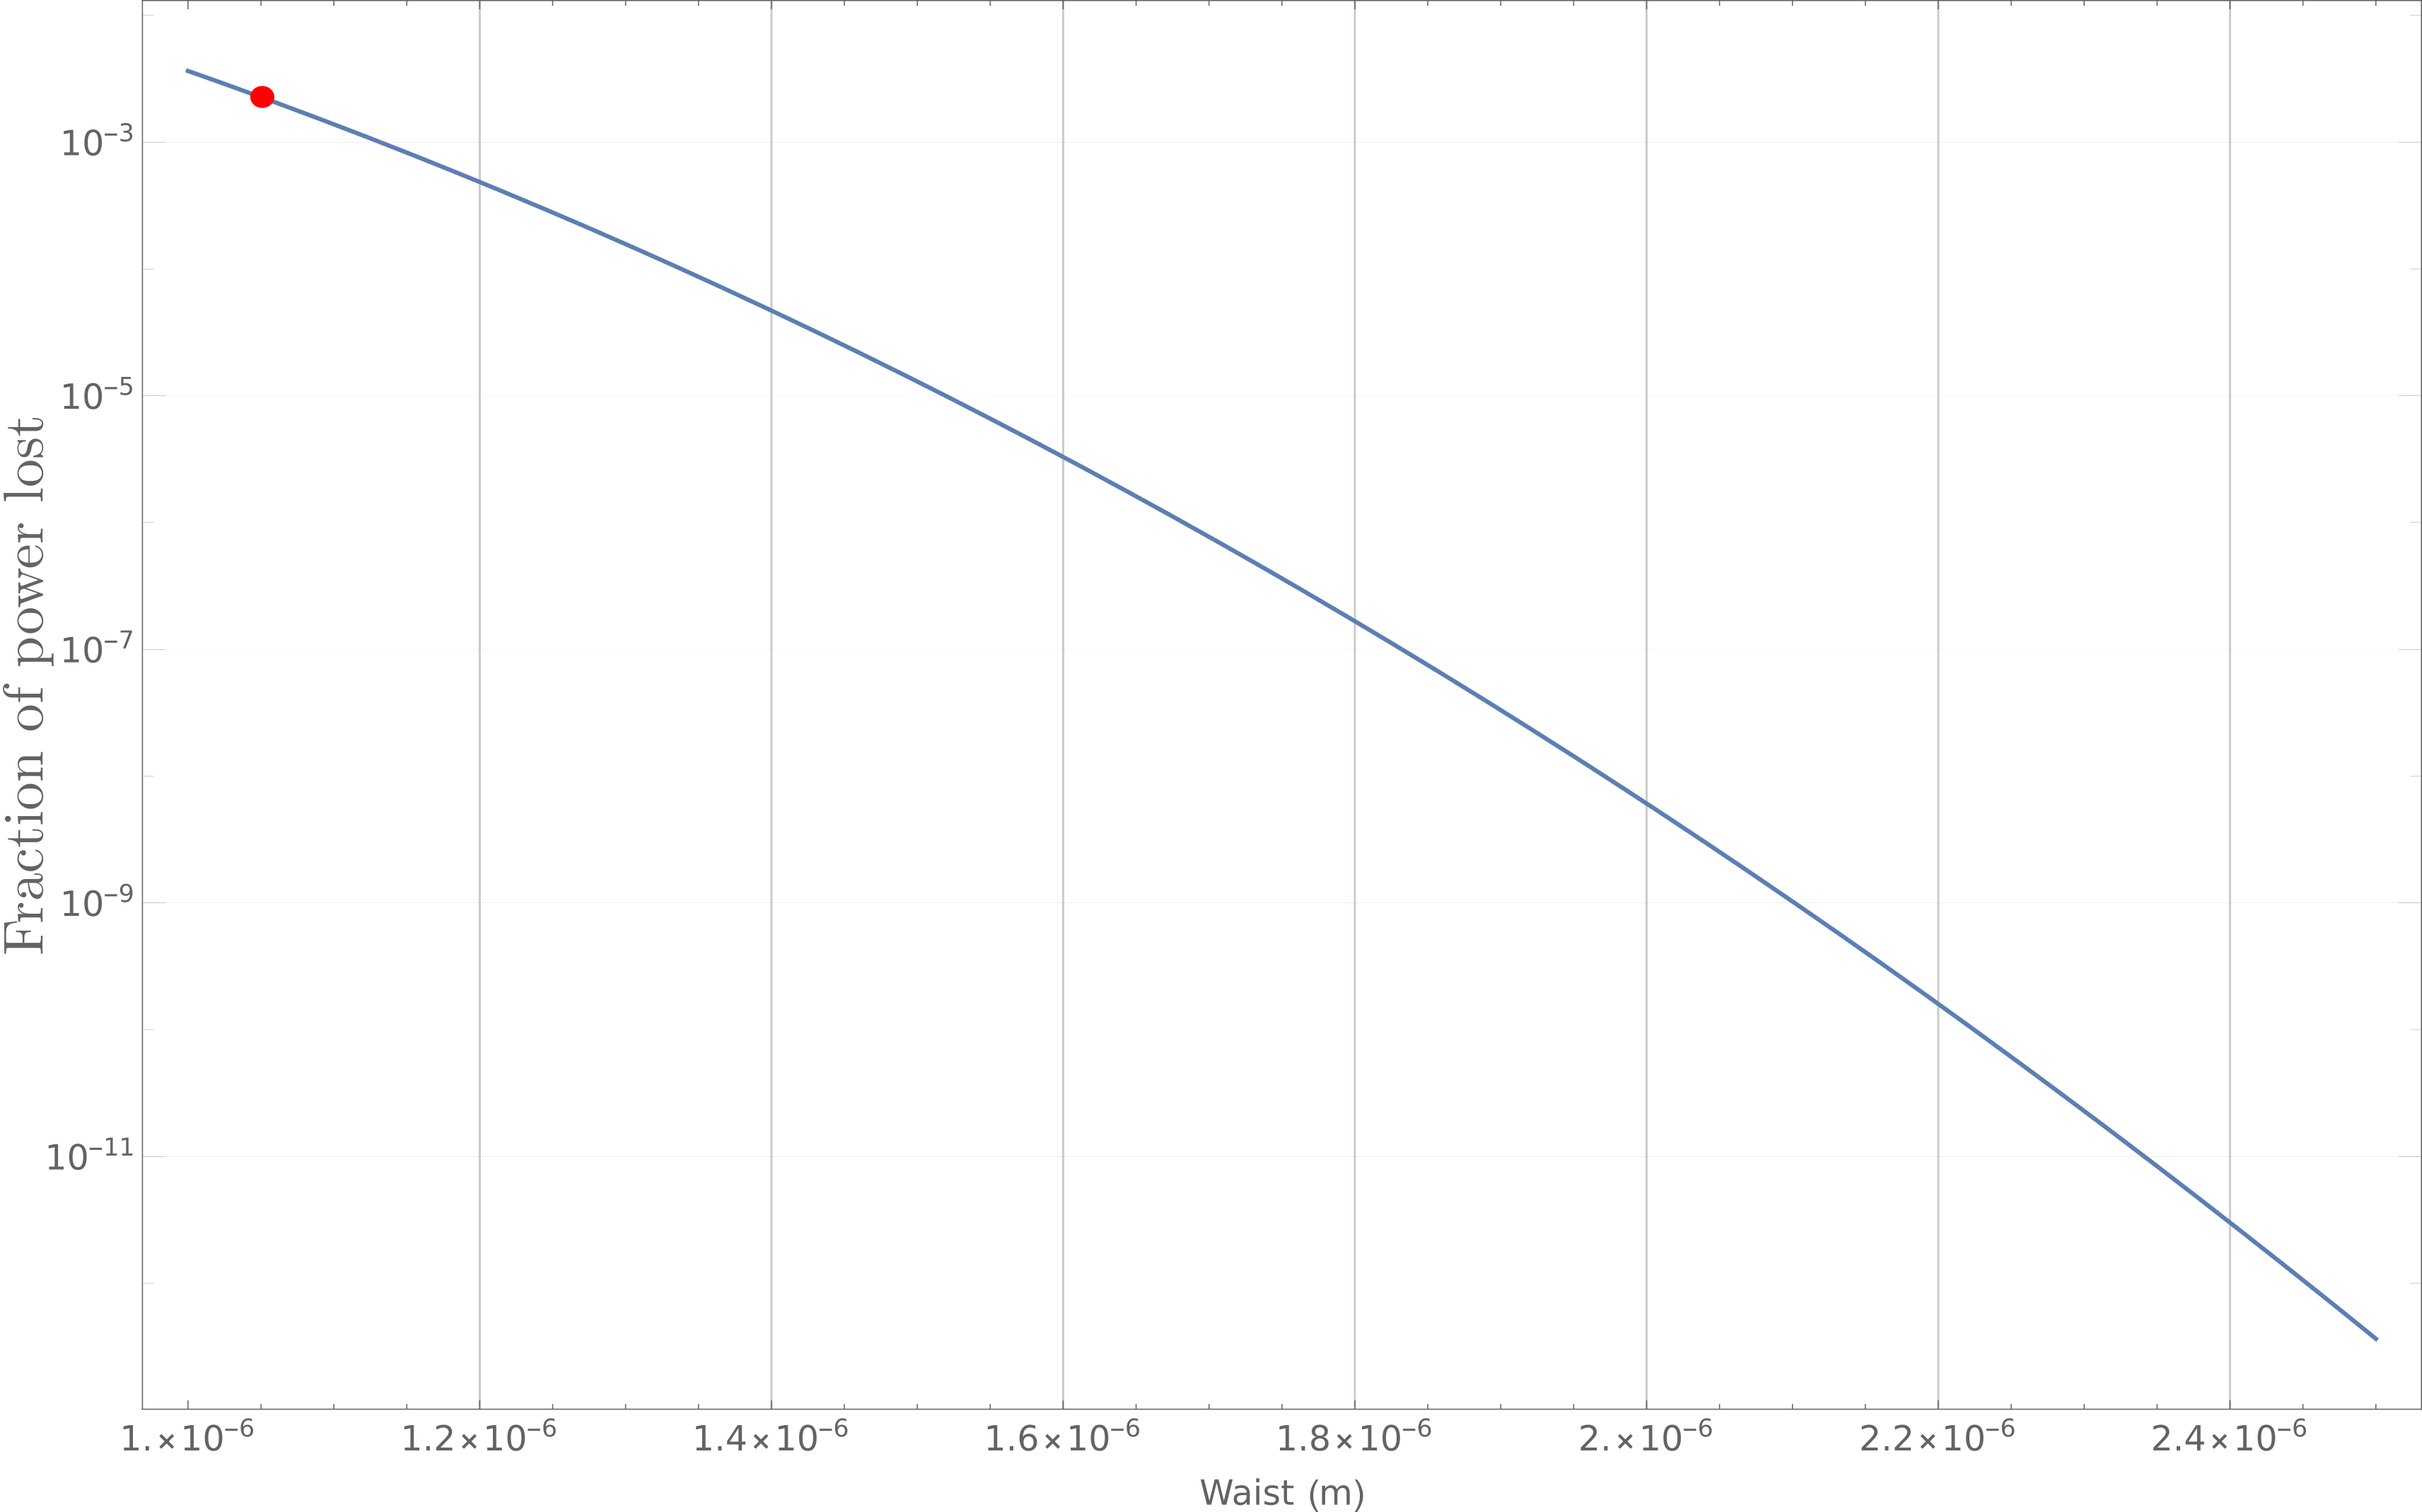
\includegraphics[width=1\textwidth]{img/powerlost}
%          \caption{Fraction of power lost due to clipping on the compensation electrodes as a function of the beam waist when focused on ion. Red point represents the waist $1.02\,\mu$m, obtained from the simulation.}
%          \label{lossesplot}
%    \end{subfigure}
% \end{figure}
\begin{figure}
       \centering
         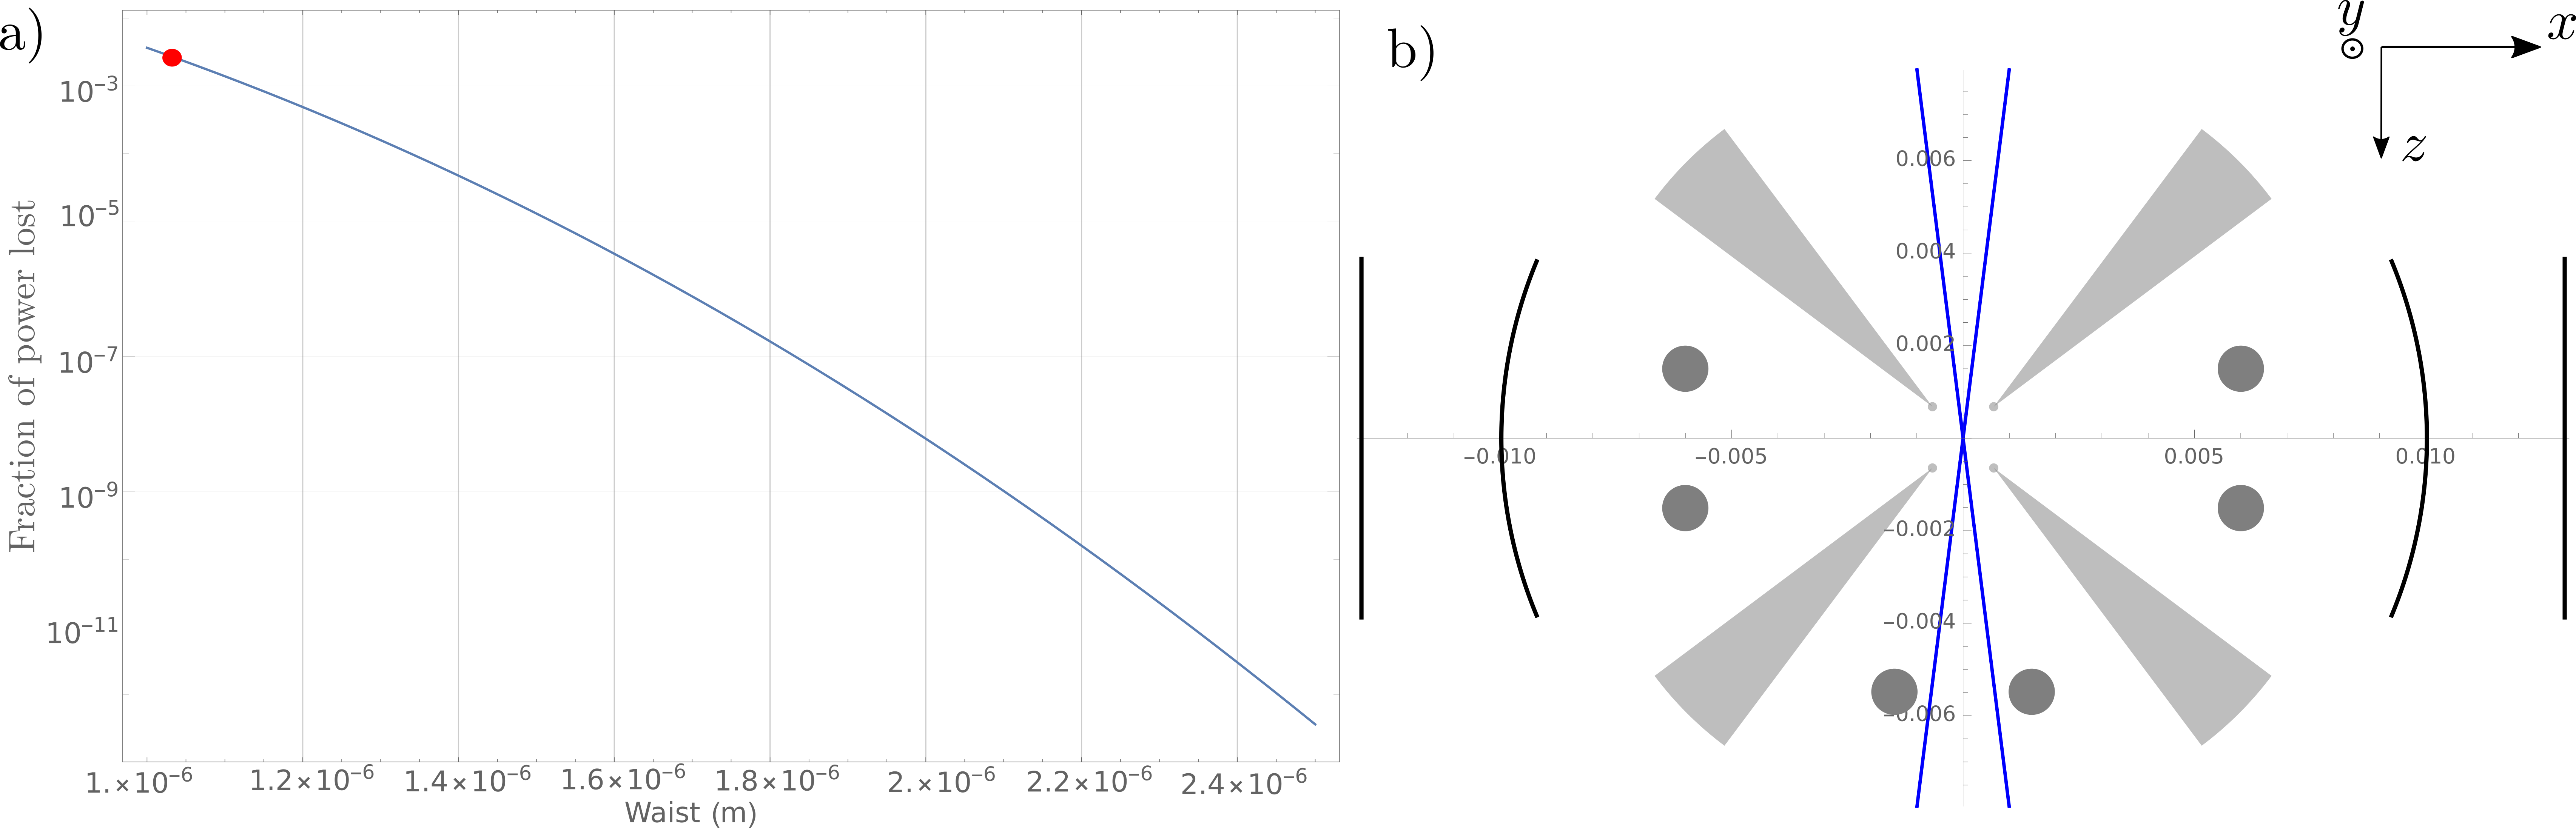
\includegraphics[width=\textwidth]{powerlost_plus_diagram}
         \caption{a) Fraction of power lost due to clipping on the compensation electrodes as a function of the beam waist when focused on ion. Red point represents the waist $1.02\,\mu$m, obtained from the simulation. b) Top view of the trap and addressing beam. Grey circles are the compensation electrodes, blue is the radius $1/e^2$ of the beam focused on the ions with waist of 1.02 $\mu$m, while the black arches represent the mirrors of the cavity. All units are in meters.}
         \label{lossesplot}
 \end{figure}

% \begin{figure}
%      \centering
%
%      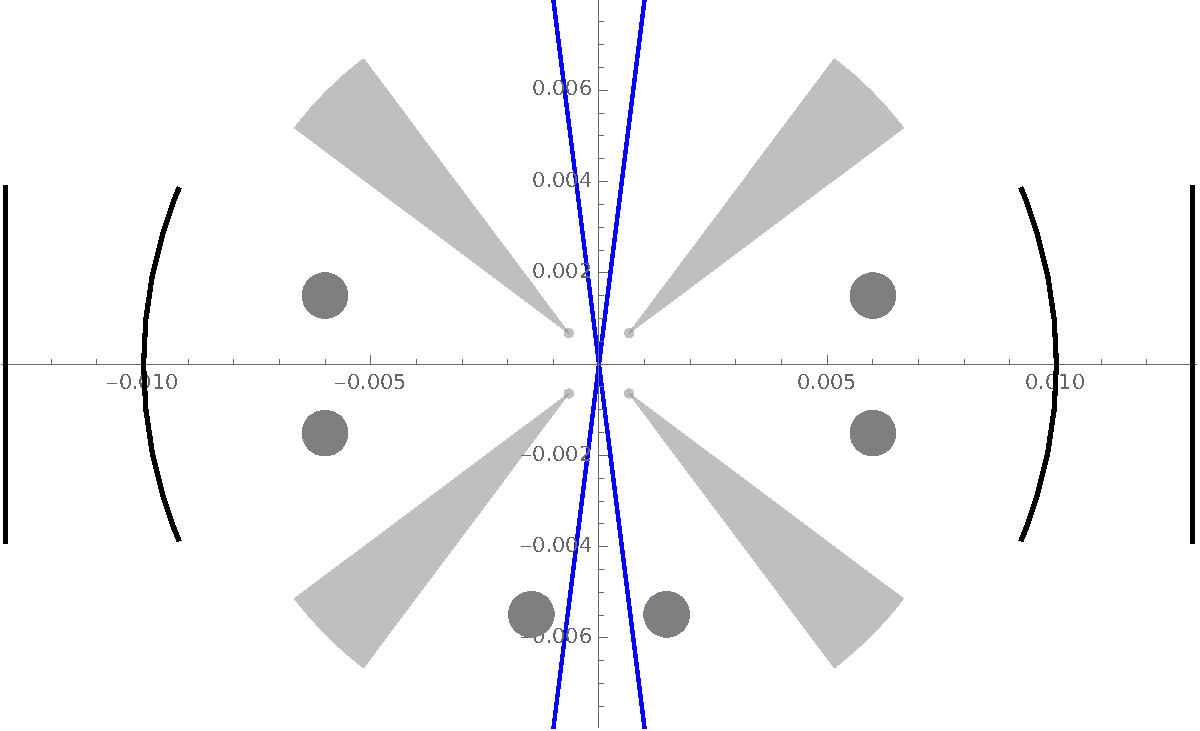
\includegraphics[width=.7\textwidth]{img/clipping}
%      \caption{Top view of the trap and addressing beam. Grey circles are the compensation electrodes, blue is the radius $1/e^2$ of the beam focused on the ions with waist of 1 $\mu$m, while the black arches represent the mirrors of the cavity.}
%      \label{clippingtop}
%      \end{figure}
% \begin{figure}
%       \centering
%         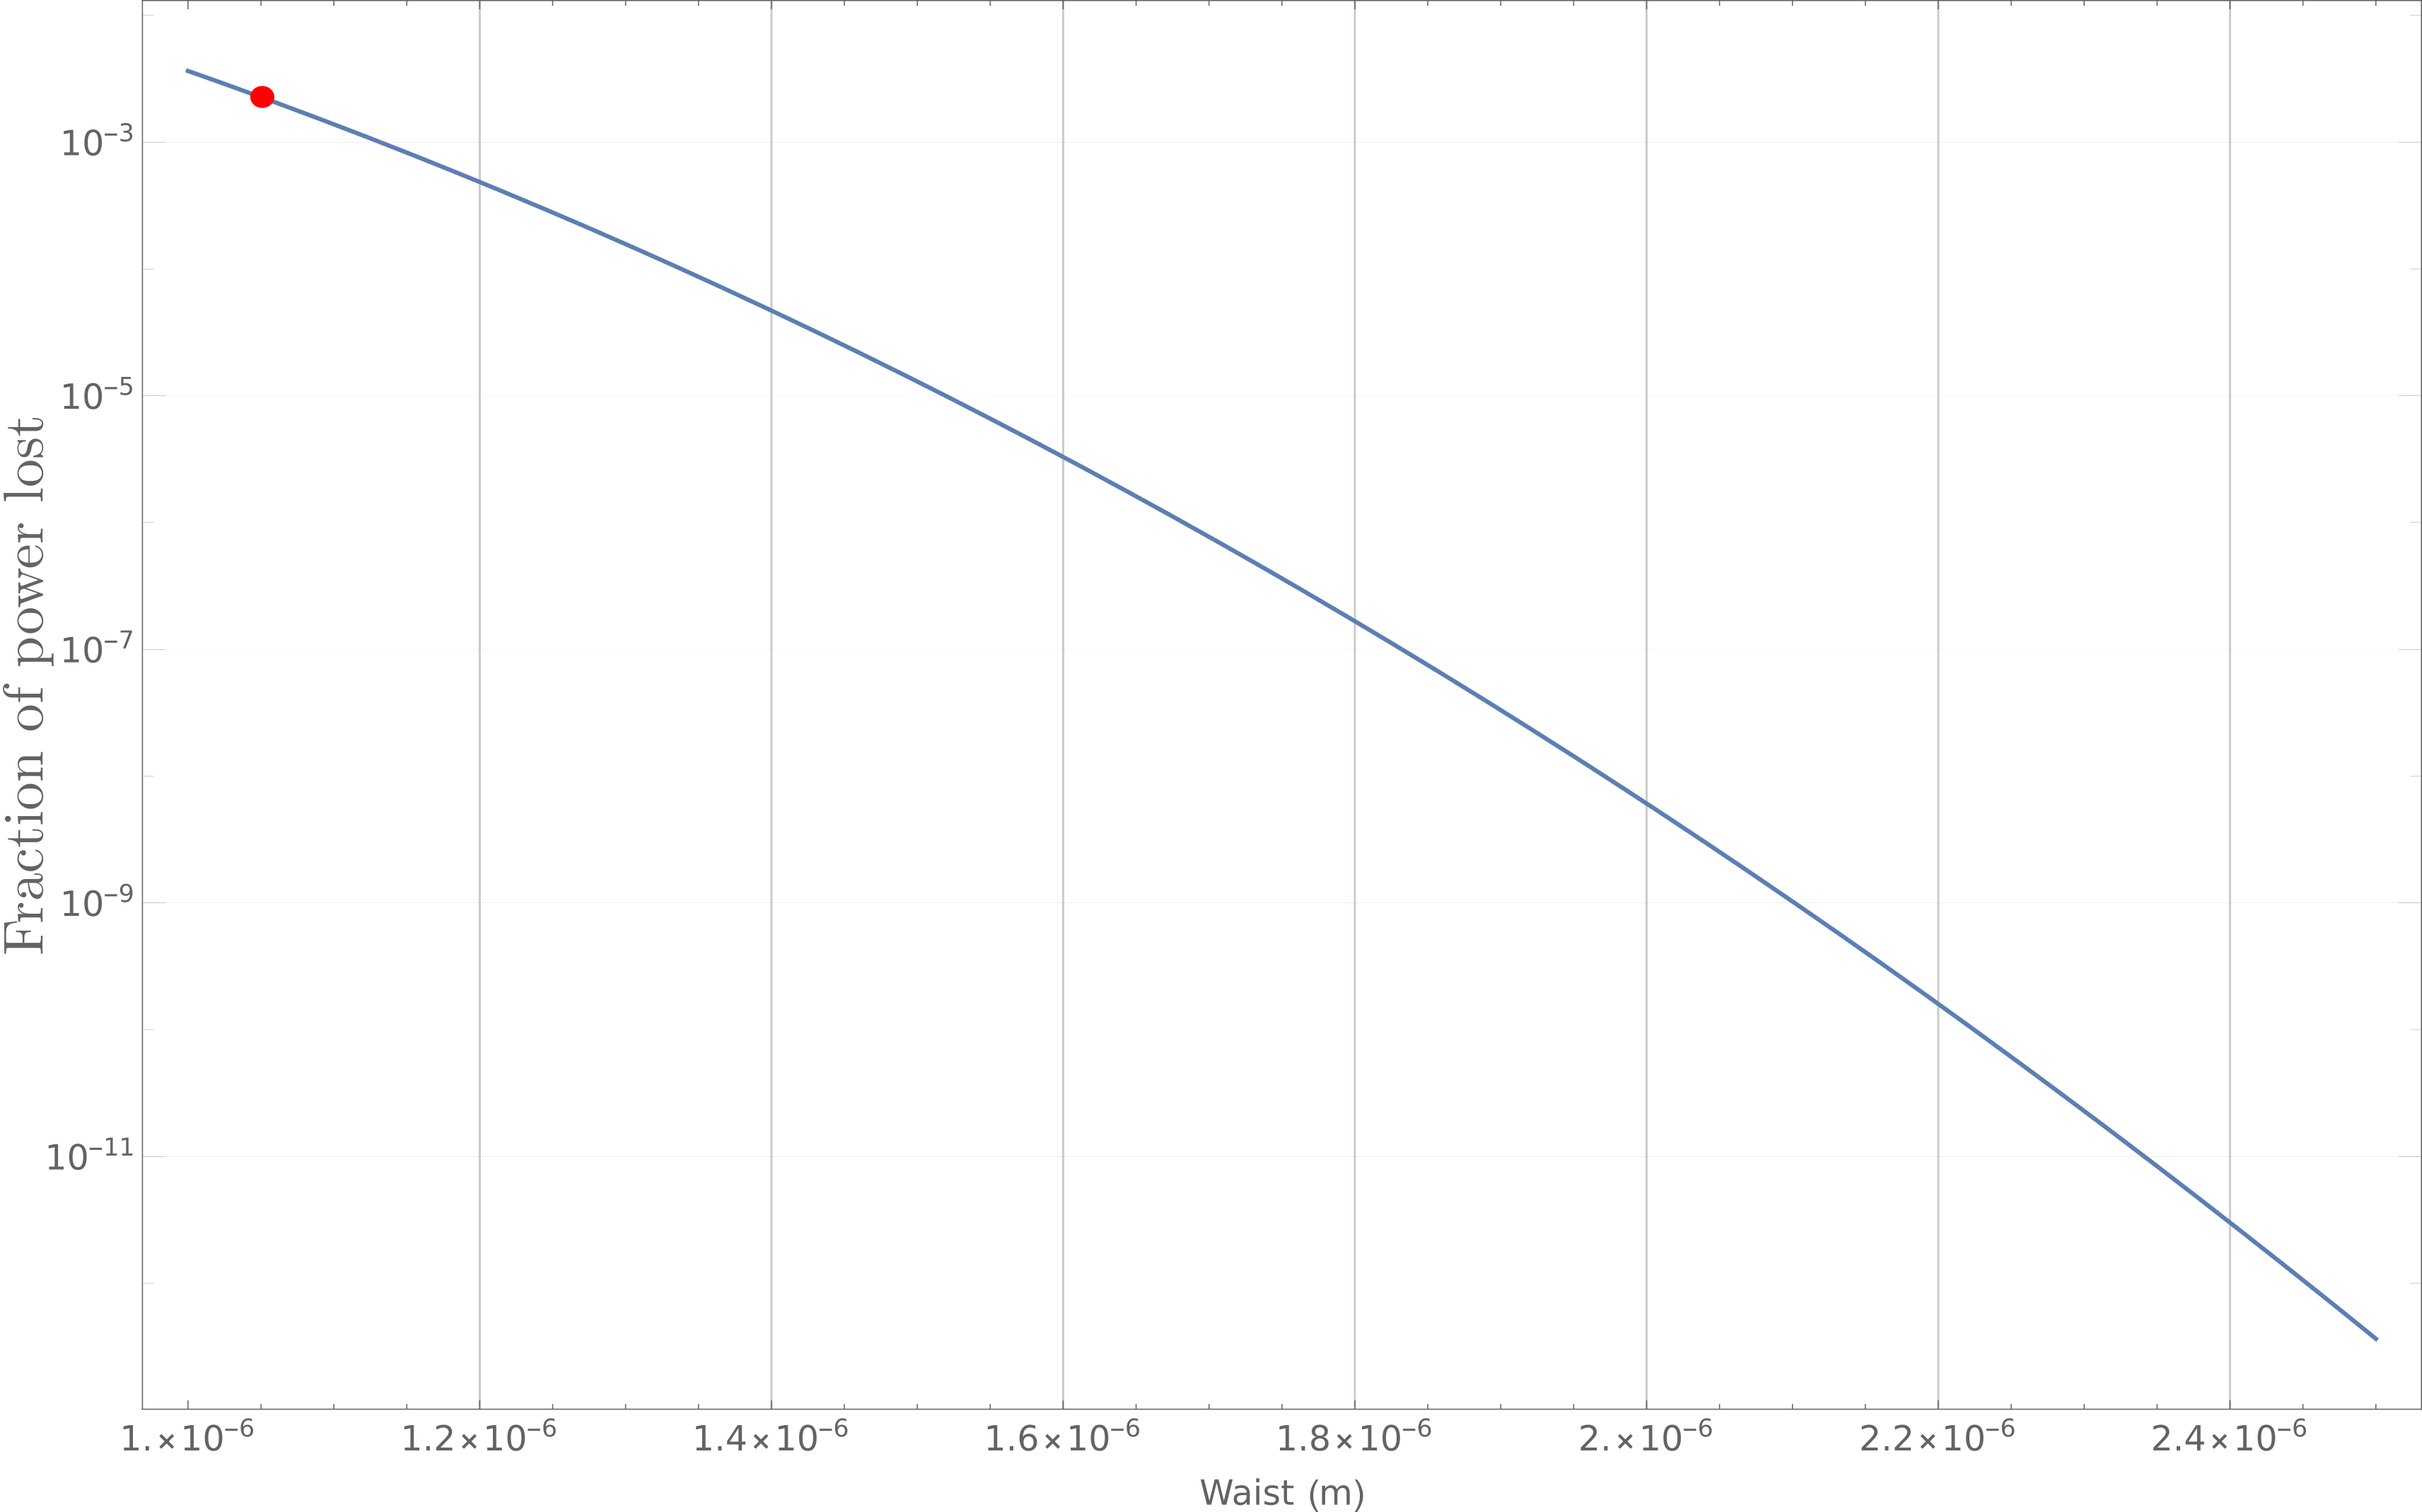
\includegraphics[width=.8\textwidth]{img/powerlost}
%         \caption{Fraction of power lost due to clipping on the compensation electrodes as a function of the beam waist when focused on ion. Red point represents the waist $1.02\,\mu$m, obtained from the simulation.}
%         \label{lossesplot}
%
% \end{figure}

To conclude this section, we discuss some aspects of the design.


\section{Physical implementation}
\label{design4}
Once the simulation gave satisfactory results, a test setup was built. The idea of building first a test setup on a different optical table from the main experiment was to check if the system was working as intended, and asses its performance. Due to physical access problems, in the final system there is no space to place a beam profiler, or a polarimeter, and after the objective there is no access to the vacuum and the trap. While on another table everything could be checked and tested. The results of the measurements obtained on this test setup are presented in chapter \ref{ch:results}.\\
Afterwards, the system was moved and implemented on the experiment optical table. For the initial alignment, a counter propagating red beam was sent in the opposite direction: starting from the front of the chamber, through the ions, and through to the objective and back through the addressing path. Since the lenses of the addressing are antireflection coated for 393 nm, the reflection of the red beam was visible and it was possible to align the components such that the beam passed approximately through the center and perpendicular to the surfaces. Calibration was also done with ions and the beam position was indirectly observed on the camera. A string of ion was used as a probe by constantly imaging the ions with 397 nm and 393 nm light on the camera. The 393 nm laser drives the transition $\text{S}_{1/2}\to \text{P}_{3/2}$, from $\text{P}_{3/2}$ the electron has two other decay channels, $\text{D}_{3/2},$ and $\text{D}_{5/2}$, which means that the electron will eventually end up in one of these two states if only the 393 nm and the 397 nm lasers are used. Repumping with 854 nm and 866 nm light the transitions $\text{D}_{5/2}\to \text{P}_{3/2}$, and $\text{D}_{3/2}\to \text{P}_{1/2}$ avoids this problem and brings the electron back to the fluorescence cycle. To observe where the 393 nm beam is, it is possible to send pulses of 854 nm light
such that, when the 854 nm light is off, the ions addressed by the 393 nm laser become dark after decaying from $\text{P}_{3/2}\to  \text{D}_{5/2}$. The ions become bright again when a new pulse of 854 nm light is sent, therefore if the pulse rate is slow enough it is possibile to see the addressed ions as blinking. This allowed to visualize the position and roughly the dimension of the 393 nm beam for the final calibration.\\
A photo of the installed system is in figure \ref{photosetup}. Here, the collimating lens is mounted on a 3D manual screw-gauge translation stage for fine tuning calibration position of the focus w.r.t. the ion string. Manual screws were later replaced with remote controlled ones from Newport, model PZA12 so that beam alignment is possible without opening the mu-metal enclosure. An iris is also used to block the zeroth order beam from the AOD. Moreover, The AOD is placed on a rotational mount that allows to tilt it in two directions. One direction was used to find the Bragg angle of the AOD to achieve maximum diffraction efficiency, and the other can be used to tilt the axis over which the AOD sweeps. This can be used to compensate for an ion string which is not exactly parallel to the AOD sweeping direction.

\begin{figure}[H]
\centering
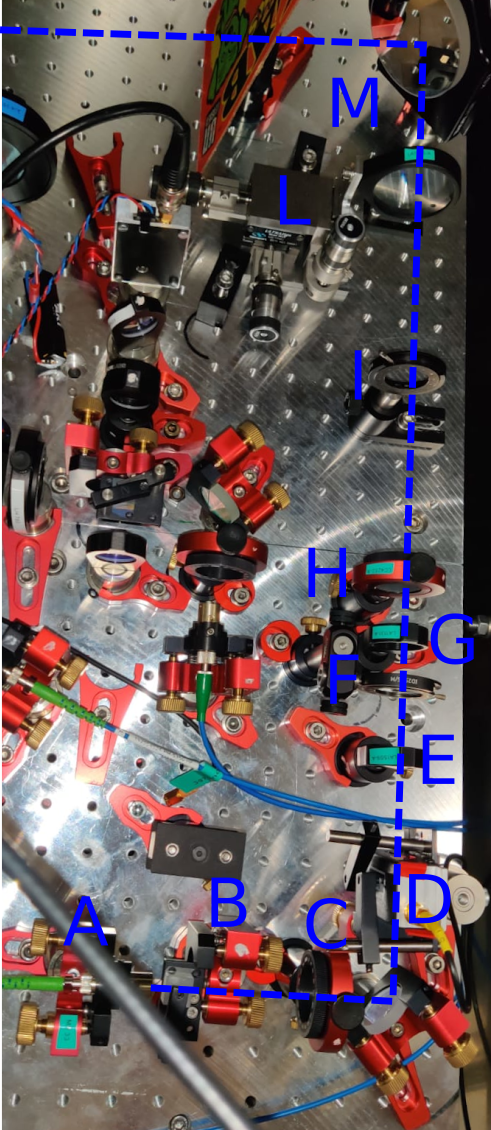
\includegraphics[scale = 1.3]{photosetupnice_withlabels.png}
\caption{Photo of the final setup. The blue dashed line is the beam path starting from bottom left at the fiber collimator, all the way to the top where a mirror deflects the beam and send it to the beam splitter. The following elements are visible: (A) Fiber collimator 60FC-M12-33 (B) Polarizing beam splitter (C) $\lambda/2$ (D) AOD (E) Lens LA-1059 (F) Iris to block 0th order (G) Lens LA-1131 (H) Diverging lens LA-4252 (I) Iris (L) Lens LA-1725 on the 3D manual screw-gauge translation stage (M) Mirror. }
\label{photosetup}
\end{figure}
